\chapter{Oefeningensessie 3}


\section{Oefening 10.1 p223}

Gegeven het volgende programma:
\begin{lstlisting}
1	m := 0
2	v := 0
3	if v >= n: 	goto 15
4	r := v
5 	s := 0
6	if r < n: 	goto 9
7	v := v + 1
8	goto 3
9	x := M[r]
10	s := s + x
11	if s <= m:	goto 13
12	m := s
13	r := r + 1
14 	goto 6
15 	return m
\end{lstlisting}

\begin{enumerate}
	\item \textbf{Teken de CFG.} (figuur \ref{fig:ex10_1p223})
	
	Dit is dezelfde graaf als degene die de basisblokken voorstelt met het enige verschil dat elke instructie nu ook een apart blok is. 
	\begin{figure}[ht]
		\centering
		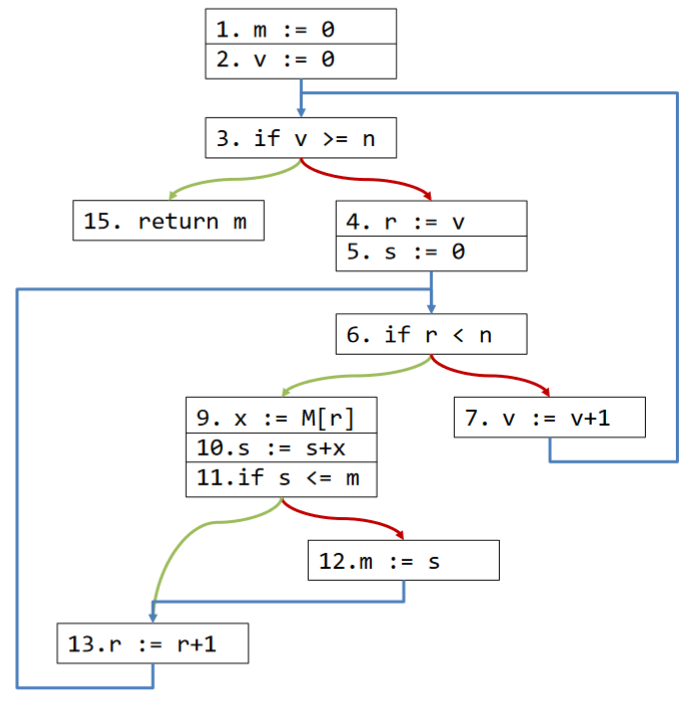
\includegraphics[width=0.7\textwidth]{ex10_1p223}
		\caption{De CFG.}
		\label{fig:ex10_1p223}
	\end{figure}
	\item \textbf{Bereken de in en out sets voor elk statement.} (tabel \ref{table:in_out_sets})
	
	Best in reverse order uitvoeren (begin vanaf laatste statement), anders kan het veel langer duren. Bereken eerst de out set, en daarna de in set want de in set is afhankelijk van de out set van dezelfde instructie.
	\begin{table}[ht]
		\begin{tabular}{| c | c c c || l l | l l|}
			\hline
			 & Succ & Use & Def & Out        & In	 & Out        & In\\
			\hline
			15         &  /   &  m  &     &            &  m      & & m\\
			13         &  6   &  r  &  r  &            &  r     &m,r,s,v,n&m,r,s,v,n\\
			12         &  13  &  s  &  m  & r          &  r,s   &m,r,s,v,n&r,s,v,n\\
			11         & 12,13& s,m &     & r,s        &  m,r,s &m,r,s,v,n&m,r,s,v,n\\
			10         &  11  & s,x &  s  & m,r,s      &  m,r,s,x&m,r,s,v,n&m,r,s,v,n,x\\
			9          &  10  &  r  &  x  & m,r,s,x    &  m,r,s &m,r,s,v,n,x&m,r,s,v,n\\
			7          &  3   &  v  &  v  &            &  v    &m,v,n&m,v,n\\
			6          & 7,9  & r,n &     & m,r,s,v    &  m,r,s,v n&m,r,s,v,n&m,r,s,v,n \\
			5          &  6   &     &  s  & m,r,s,v,n  &  m,r,v,n&m,r,s,v,n&m,r,v,n\\
			4          &  5   &  v  &  r  & m,r,v,n    &  m,v,n&m,r,v,n&  m,v,n\\
			3          & 4,15 & v,n &     & m,v,n      &  m,v,n & m,v,n&  m,v,n   \\
			2          &  3   &     &  v  & m,v,n      &  m,n   & m,v,n &  m,n  \\
			1          &  2   &     &  m  & m,n        &  n     & m,n &  n\\
			\hline
		\end{tabular}
	\hfill
	\begin{tabular}{|c|cccccc|}
		\hline
		& m &r & s & v & n & x \\
		\hline
		m &   &x & x & x & x & x \\
		r &   x& & x & x & x & x \\
		s &   x&x &  & x & x & x \\
		v &   x&x &  x&  & x & x \\
		n &   x&x & x & x &  & x \\
		x &   x&x &  x& x & x &  \\
		\hline
	\end{tabular}
		\caption{De in en out sets + de interferentiematrix.}
		\label{table:in_out_sets}
	\end{table}
	\item \textbf{Teken de register-interferentiegraaf.} (tabel \ref{table:in_out_sets})
	

\end{enumerate}



\newpage
\section{Oefening 11.3 p263}
Beschouw de graaf op figuur \ref{fig:ex11_3p263}. De volle lijnstukken stellen interferenties voor en de gestreepte lijnen een \texttt{MOVE}.
\begin{figure}[ht]
	\centering
	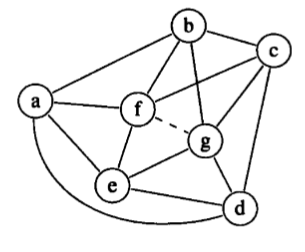
\includegraphics[width=0.5\textwidth]{ex11_3p263}
	\caption{}
	\label{fig:ex11_3p263}
\end{figure}

\begin{enumerate}
	\item \textbf{Kleur de graaf zonder \textit{coalescing} en $k = 4$. Toon de \textit{select}-stack die de volgorde aangeeft waarin knopen verwijderd worden. Is er een potentiële \textit{spill}? Is er een echte \textit{spill}?} (Figuur \ref{fig:ex11_3p263_partone})
	\begin{figure}
		\centering
		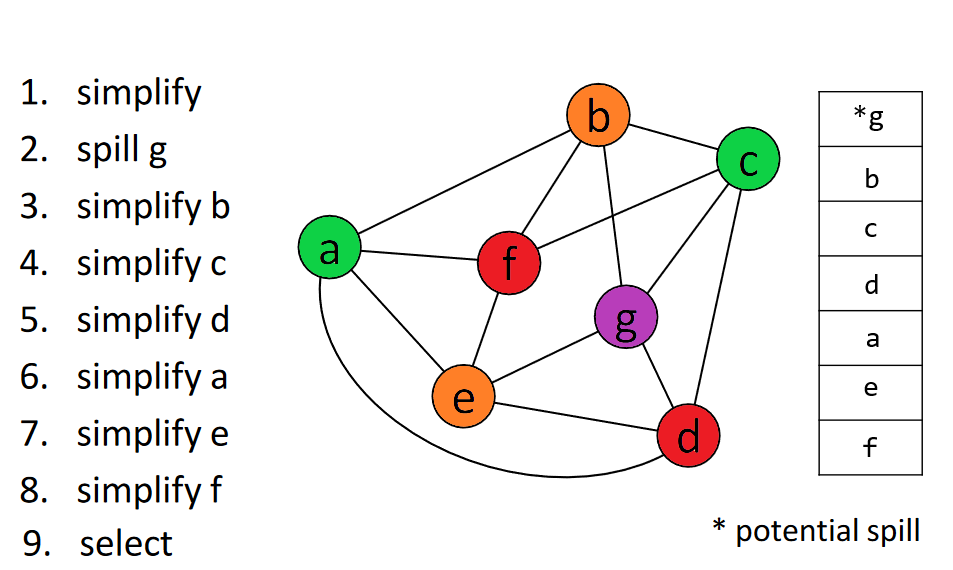
\includegraphics[width=0.5\textwidth]{ex11_3p263_partone}
		\caption{}
		\label{fig:ex11_3p263_partone}
	\end{figure}
	De knoop $g$ was een potentiële spill, maar de graaf kon nog steeds helemaal gekleurd worden dus was het geen echte spill.
	\item \textbf{Kleur de graaf met \textit{conservative coalescing} en $k = 4$. Wanneer wordt Briggs of George gebruikt?  Is er een potentiële \textit{spill}? Is er een echte \textit{spill}?}
\end{enumerate}


\newpage
\section{Oefening 17.5 p408 (licht gewijzigd)}
Gegeven het volgende programma:
\begin{lstlisting}
1.  y := x
2.  z := 1
3.  if y == 0: goto 7
4.  z := z * y
5.  y := y - 1
6.  goto 3
7.  y := 0
\end{lstlisting}

\begin{enumerate}
	\item \textbf{Teken de CFG.} (Figuur \ref{fig:ex17_5p408_cfg})
	\begin{figure}[ht]
		\centering
		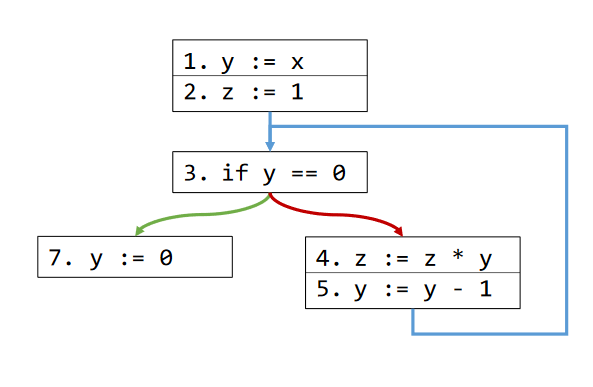
\includegraphics[width=\textwidth]{ex17_5p408_cfg}
		\caption{De CFG.}
		\label{fig:ex17_5p408_cfg}
	\end{figure}
	\item \textbf{Bereken de \textit{reaching definitions} waarbij het resultaat van elke iteratie getoond wordt. Hoeveel iteraties zijn er nodig.}
	Er zijn 3 iteraties nodig (want laatste iteratie verandert niets meer). (Tabel \ref{table:reaching_definitions})
	\begin{table}[ht]
		\centering
		\begin{tabular}{| c | c c c || l l | l l|}
			\hline
				& Pred 	& Gen 	& Kill 	&	In	&	Out		&	In 	&	Out		\\
			\hline
			1	&	/	&	1	&	5,7	&	/	&	1		&	/	&	1		\\
			2	&	1	&	2	&	4	&	1	&	1,2		&	1	&	1,2		\\
			3	&	2,5	&	/	&	/	&	1,2	&	1,2		&1,2,4,5&	1,2,4,5	\\
			4	&	3	&	4	&	2	&	1,2	&	1,4		&1,2,4,5&	1,4,5	\\
			5	&	4	&	5	&	1,7	&	1,4	&	4,5		&1,4,5	&	4,5		\\
			7	&	3	&	7	&	1,5	&	1,2	&	2,7		&1,2,4,5&	2,4,7		\\
			\hline
		\end{tabular}
		\caption{De reaching definition tabel.}
		\label{table:reaching_definitions}
	\end{table}
\end{enumerate}